\chapter{Étude d'un système de transport}
Dans cette première partie, nous allons vous présenter nos travaux sur l'étude d'un système de transport. Dans ce problème, il nous est demandé de mettre en œuvre, avec l'algèbre $(max,+)$, une étude d'un système de GET qui représentera notre système temporisé de transport. Nous commencerons par vous présenter le graphe d'évènements correspondant au procédé étudié, nous effectuerons une analyse de ce système pour enfin essayer d'améliorer le système en modifiant le graphe.

\section{Graphes d'évènements temporisés}
Dans un premier temps, nous avons réalisé le graph des événements temporisés (voir figure \ref{fig:get_train}). Ce graph représente les différentes gares, un couple de transition $(x \theta1,x\theta2)$ représente la gare $\theta$, la première représente "le train rentre en gare", le $t_a$ de la place suivante le temps d'attente en gare, et la seconde transition ($x\theta2$) "le train sort de la gare". Les $ta$ des places entre deux entrées ou sorties de gare représentent le temps de trajet sur une ligne de train. Les places $xB12$ et $xB22$ sont des copies  de $xB1$ et $xB2$ afin de représenter les contraintes de synchronisation décritent dans l'énoncé.
Afin de permettre une mise en représentation qui suivra, nous avons décomposé la place $p0$ et la transition $xA2$ en deux places $p0$ et $p18$ et deux transitions $xA2$ et $xA22$. Nous avons réparti les jetons sur les deux places. Cela nous permettra de décrire les places suivantes avec un état de plus et mais uniquement par rapport à un événement précédent ("$x(k)=Yx(k-1)$") et non deux ("$x(k)=Yx(k-2)$").
Voici la nouvelle représentation d'état correspondant à cette contrainte, figure \ref{fig:get_train_decompo}.
\begin{figure}[!ht]
\centering
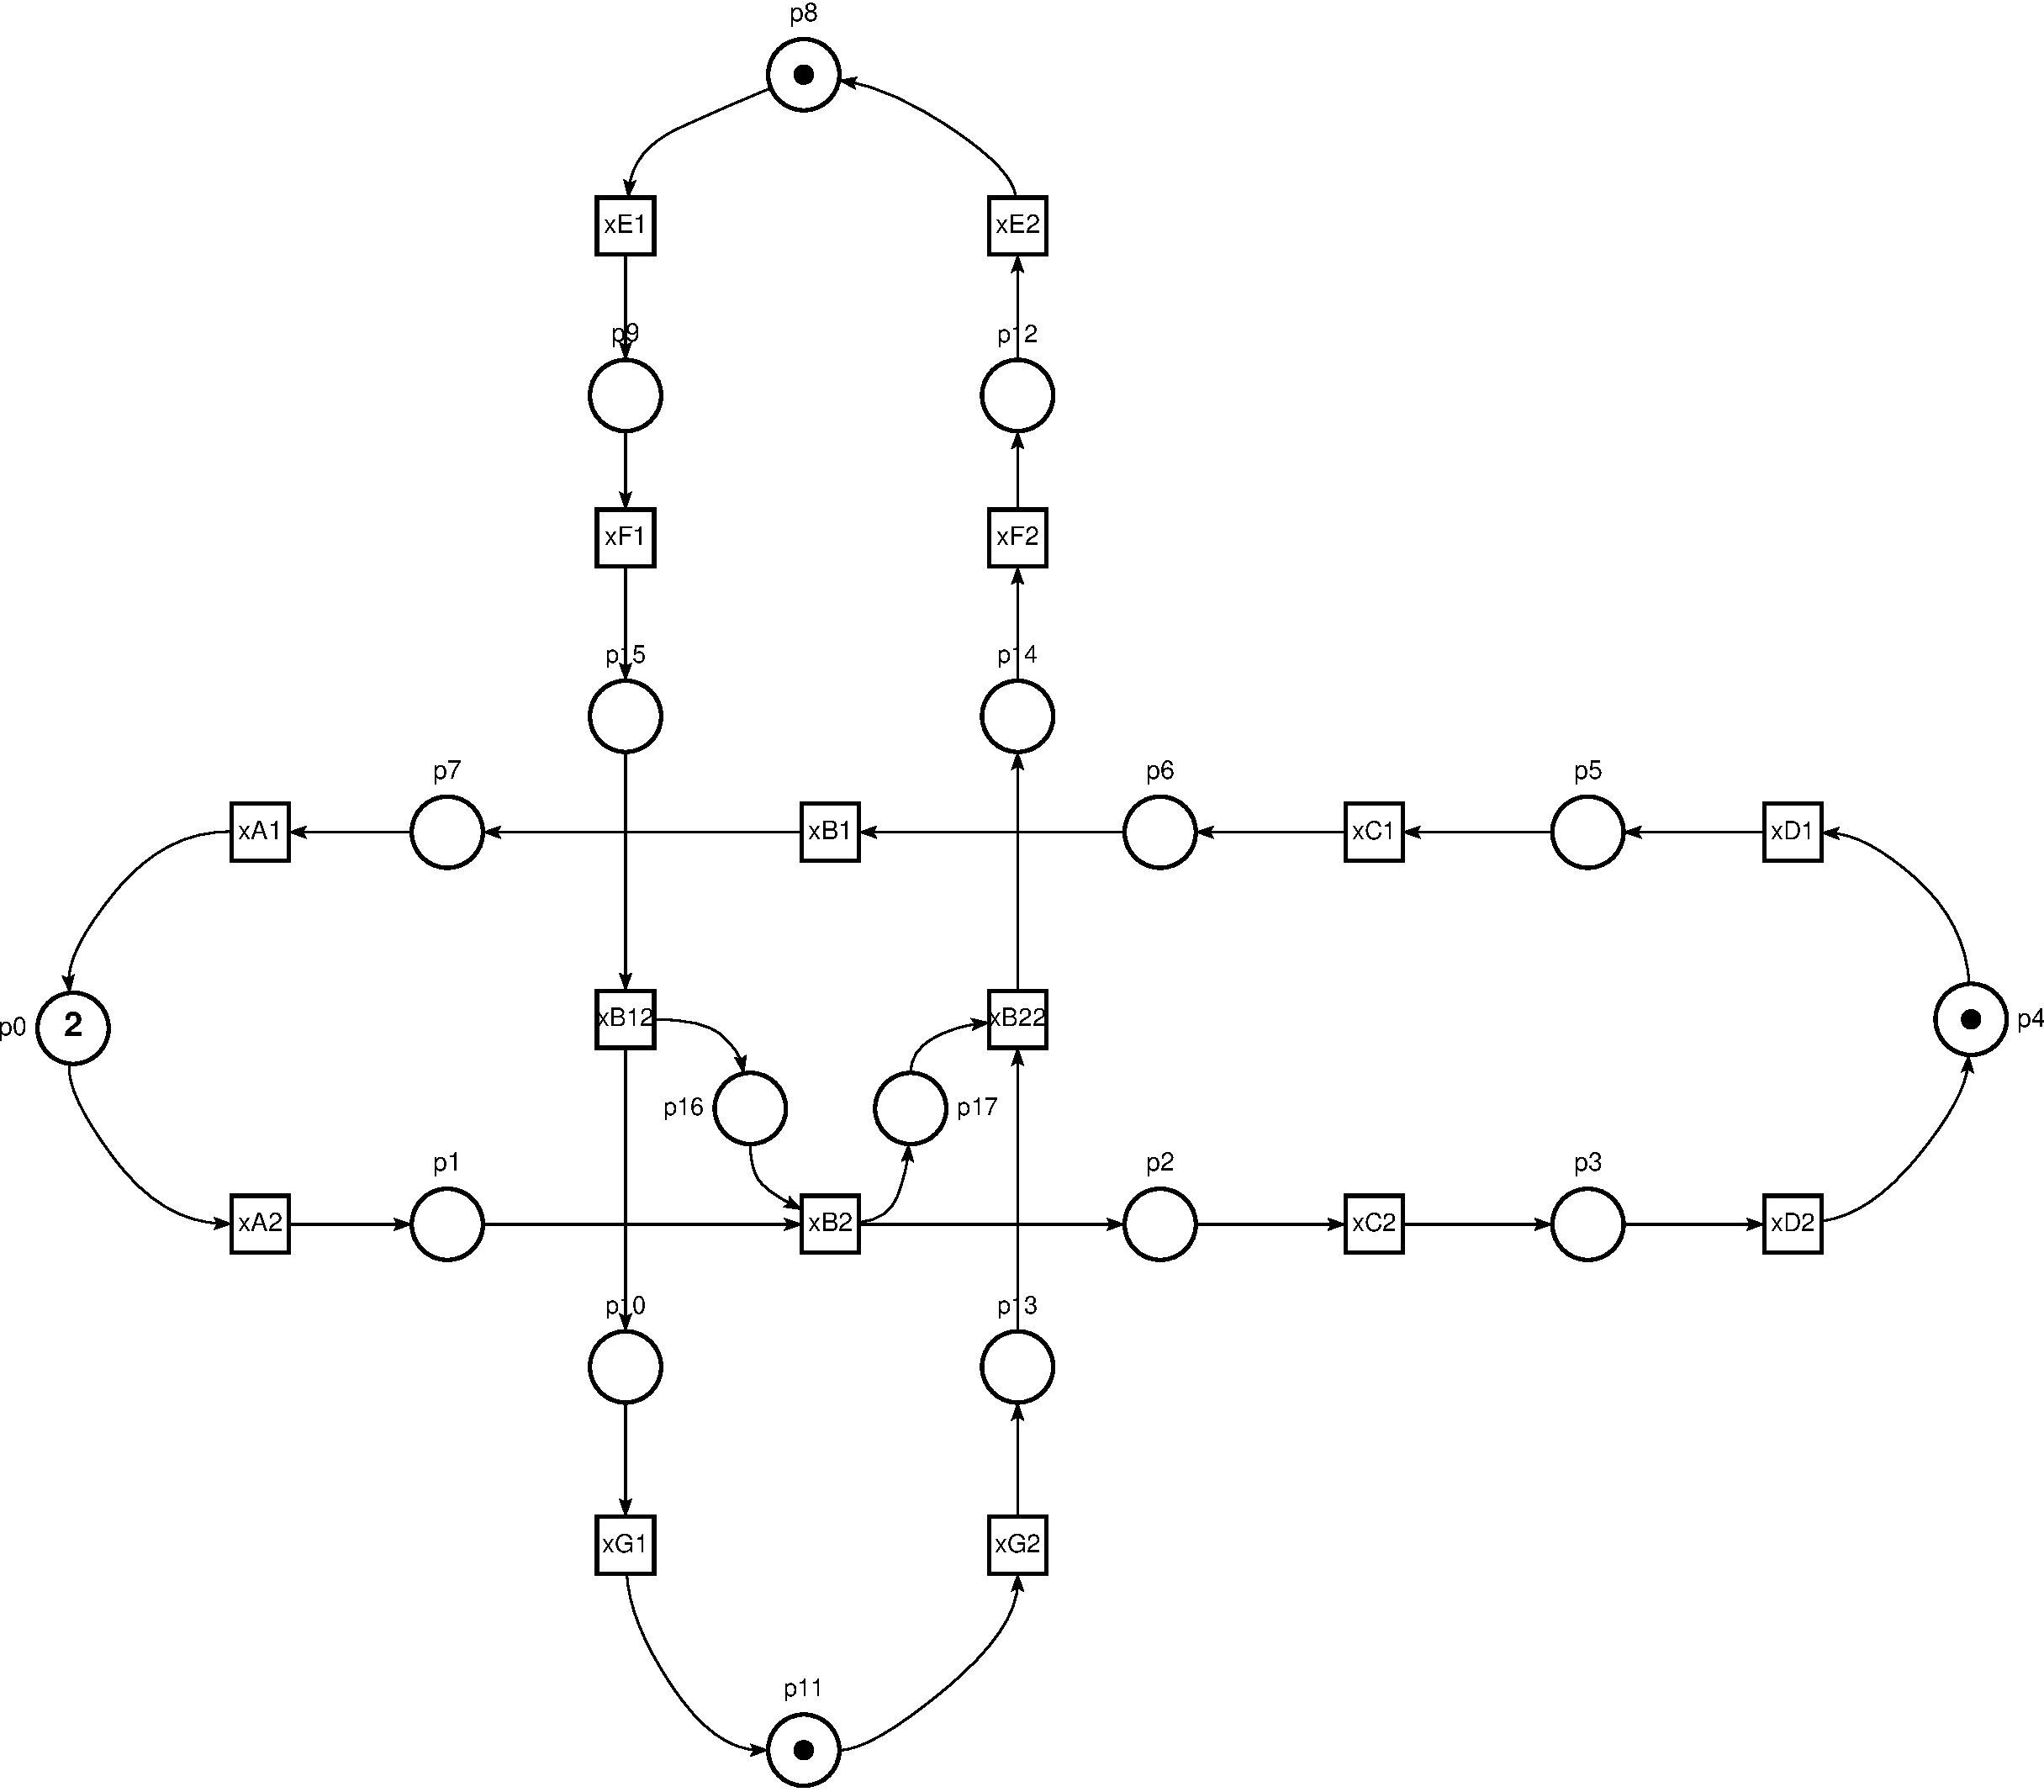
\includegraphics[width =.8 \textwidth]{./I/images/train.pdf}
\caption{\label{fig:get_train} Graphe des Événements Temporisé du réseau de transport}
\end{figure}


\begin{figure}[!ht]
\centering
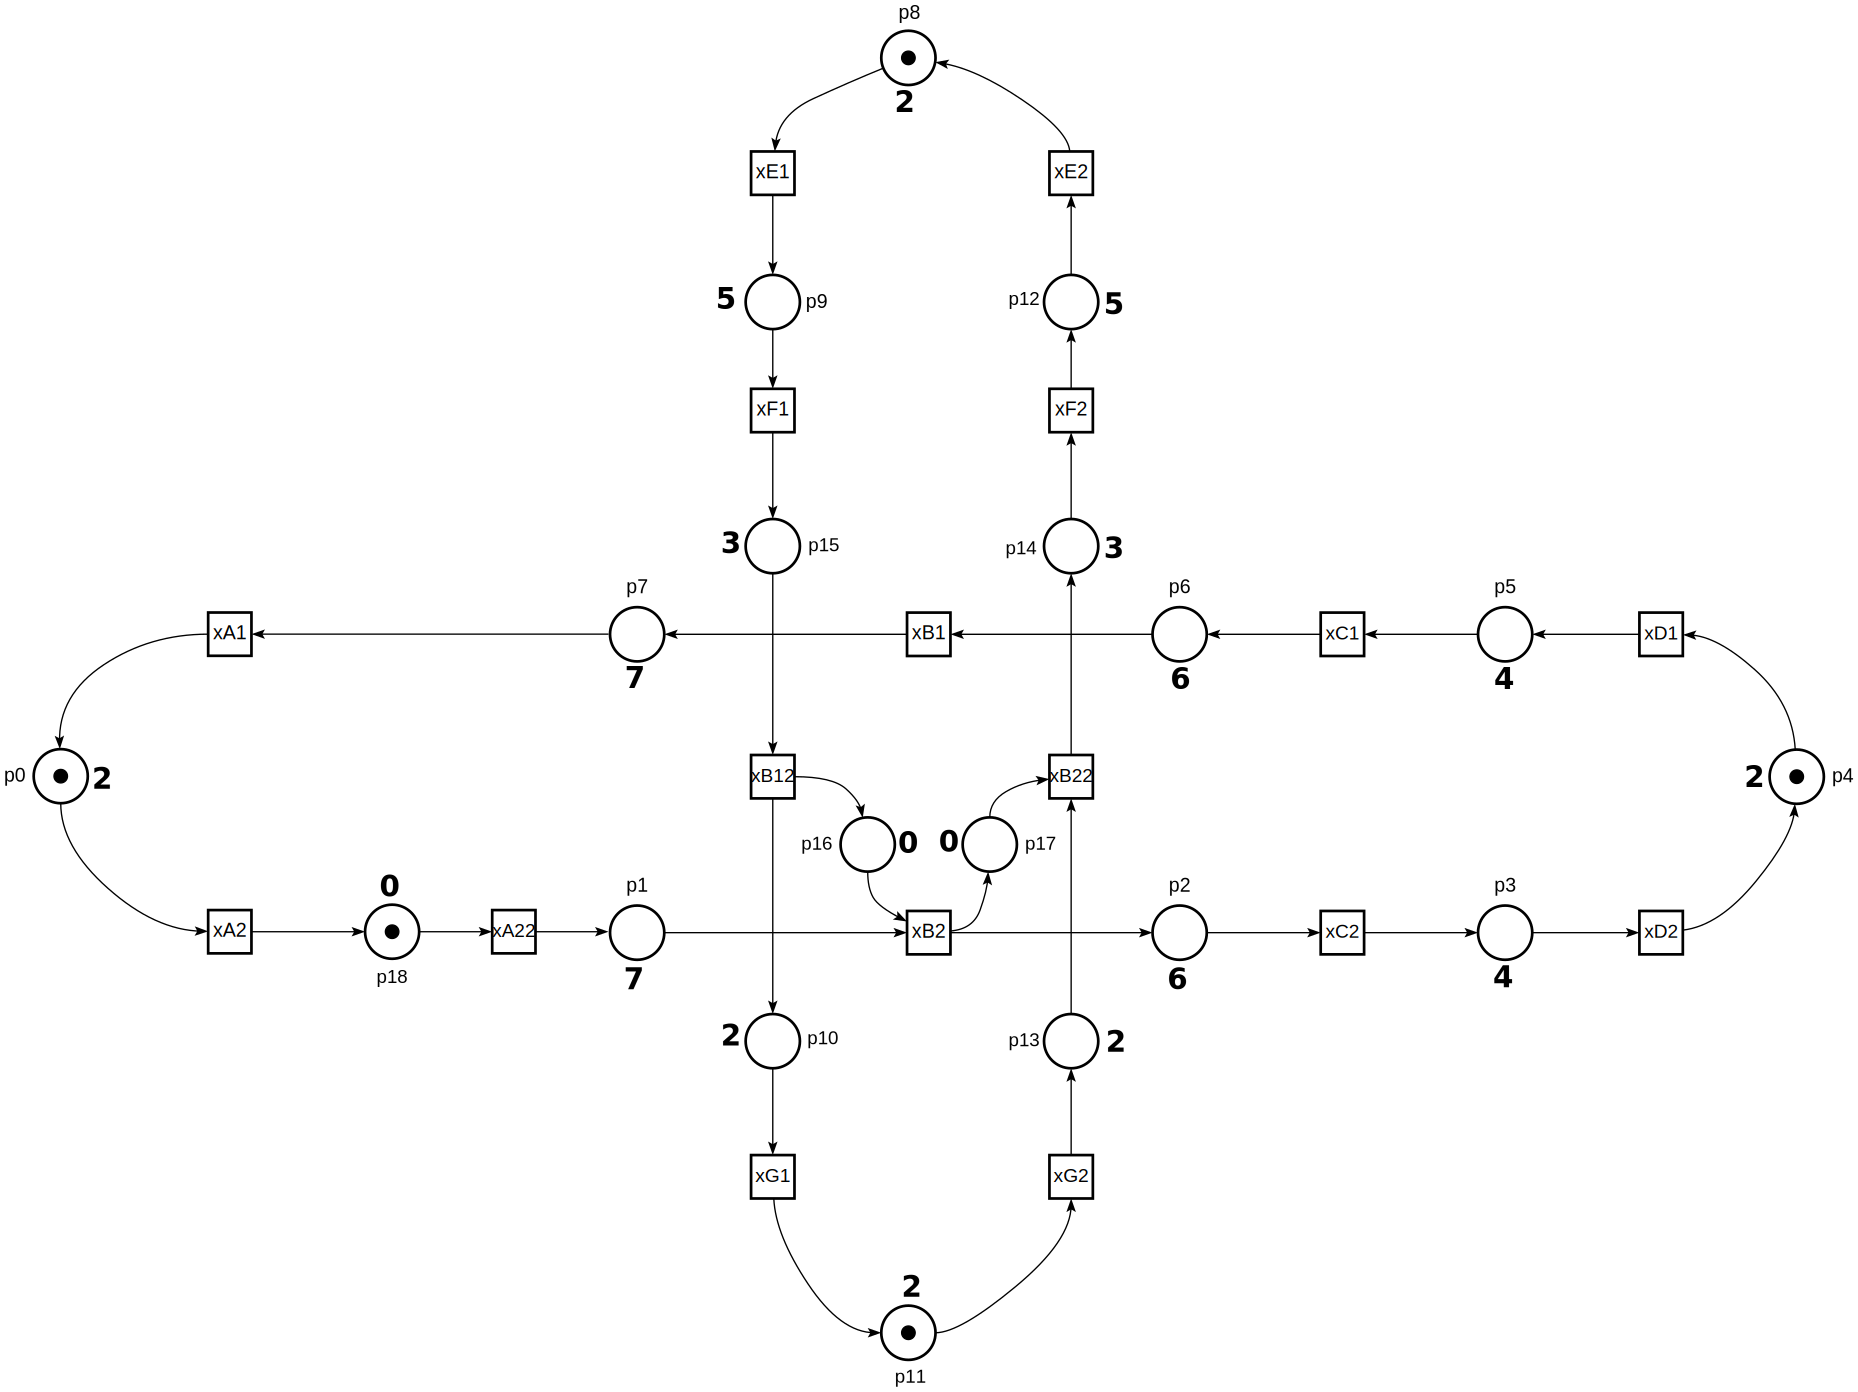
\includegraphics[width = .8\textwidth]{./I/images/train_decompose.pdf}
\caption{\label{fig:get_train_decompo} Graphe des Événements Temporisé décomposé du réseau de transport }
\end{figure}
\section{Analyse, matrice d'évolution et valeurs propres}
Nous abordons ici, dans l'ordre, la mise en représentation d'état du réseau de transport, l'analyse de réductibilité et le calcul des valeurs et vecteurs propres. 
\subsection{Représentation d'état}
Afin de réaliser la mise en représentation d'état, nous avons extrait les égalisés suivantes :
\begin{align*}
\left\lbrace
\begin{array}{l c l}
x_{A1}(k) &=&	7x_{B1}(k)\\ 
x_{B1}(k) &=&	6x_{C1}(k)\\
x_{D1}(k) &=&	2x_{D2}(k-1)\\
x_{D2}(k) &=&	4x_{C2}(k)\\
x_{C2}(k) &=&	6x_{B1}(k)\\
x_{B2}(k) &=&	7x_{A2}(k) \oplus x_{B12}\\
x_{A2}(k) &=&	2x_{A1}(k-2)\\
x_{A22}(k) &=&	x_{A1}(k-1)\\
x_{E1}(k) &=&	2x_{E2}(k-1)\\
x_{F1}(k) &=&	5x_{E1}(k)\\
x_{B12}(k) &=&	3x_{F1}(k)\\
x_{G1}(k) &=&	2x_{B12}(k)\\
x_{G2}(k) &=&	2x_{G1}(k-1)\\
x_{B22}(k) &=&	2x_{G2}(k) \oplus x_{B2}(k)\\
x_{F2}(k) &=&	3x_{B22}(k)\\
x_{E1}(k) &=&	5x_{F2}(k)   \\  
\end{array}
\right.
\end{align*}
On peut remarquer que notre système est autonome, c'est-à-dire qu'il ne présente pas d'entrée ou de sortie 
dans l'espace d'état suivant, les matrices $B$ et $C$ ne sont donc pas nécessaires.
\begin{equation}
\left\lbrace
\begin{array}{lcl}
	x(k) &=& A_0 \cdot x(k) + A_1 \cdot x(k-1) + B u(k)\\
	y(k) &=& C \cdot x(k)
\end{array}
\right. \Leftrightarrow
\left\lbrace\begin{array}{lcl}
	x(k) &=& A \cdot x(k-1)
\end{array}\right.
\end{equation}
Ces égalités nous ont permis de créer la matrice dynamique suivante : 
\begin{equation}
A = \left(\begin{array}{ccccccccccccccccc}
.&.&.&.&19&.&.&.&.& .&.&.&.& .&.&.&. \\
.&.&.&.&12&.&.&.&.& .&.&.&.& .&.&.&. \\
.&.&.&.&6& .&.&.&.& .&.&.&.& .&.&.&. \\
.&.&.&.&2& .&.&.&.& .&.&.&.& .&.&.&. \\
.&.&.&.&.& .&.&.&19&.&.&.&.& .&.&.&20\\
.&.&.&.&.& .&.&.&15&.&.&.&.& .&.&.&16\\
.&.&.&.&.& .&.&.&9& .&.&.&.& .&.&.&10\\
.&.&.&.&.& .&.&.&2& .&.&.&.& .&.&.&.\\
0&.&.&.&.& .&.&.&.& .&.&.&.& .&.&.&. \\
.&.&.&.&.& .&.&.&.& .&.&.&.& .&.&.&2 \\
.&.&.&.&.& .&.&.&.& .&.&.&.& .&.&.&7 \\
.&.&.&.&.& .&.&.&.& .&.&.&.& .&.&.&10\\
.&.&.&.&.& .&.&.&.& .&.&.&.& .&.&.&12\\
.&.&.&.&.& .&.&.&.& .&.&.&2& .&.&.&. \\
.&.&.&.&.& .&.&.&9& .&.&.&4& .&.&.&8 \\
.&.&.&.&.& .&.&.&12&.&.&.&7& .&.&.&11\\
.&.&.&.&.& .&.&.&17&.&.&.&12&.&.&.&18
\end{array}\right)
\end{equation}
($.$ signifie $\epsilon$)
\subsection{Irréductibilité}
Maintenant que nous avons une représentation d'état de notre procédé, nous allons étudier s'il est irréductible ou non, si c'est le cas, cela signifie qu'il a une unique valeur propre (c'est une implication et non une équivalence). Une des méthodes de vérification de la propriété d'irréductibilité d'une matrice est de vérifier si elle comporte une ligne ou une colonnes d'éléments neutres ($\epsilon$).
Nous pouvons voir ici que la matrice A comporte au moins 12 colonnes d'éléments neutres, elle est donc réductible. Une des autres façon est de voir si le graphe des marquages accessible est fortement connexe ou non. Si il n'est, elle est irréductible. Figure \ref{fig:gma_train}, on peut voir que ce n'est pas le cas les états 2, 3, 4, 6, 7, 8, 10, 11, 12, 14, 15 et 16 sont des états puits.
\begin{figure}[!ht]
\centering
\includegraphics[width = .4\textwidth]{./I/images/GMA.png}
\caption{\label{fig:gma_train} Graphe des Marquages accessibles de $A$}
\end{figure}
\subsection{Valeur propre}
Nous avons calculé la valeur propre à l'aide de ScicosLab, elle est unique est vaux 18. Cela veut dire que le cycle interne du système est de 18 événements une fois le régime permanent établi.
\subsection{Vecteur propre}
Comme précédemment, nous avons utilité ScicosLab pour calculer le vecteur propre de $A$.
\section{Commande des conditions initiales}


